%% Author_tex.tex
%% V1.0
%% 2012/13/12
%% developed by Techset
%%
%% This file describes the coding for rsproca.cls

\documentclass[]{cik}%%%%where rsos is the template name

\usepackage{color}
\usepackage{fancyvrb}
\newcommand{\VerbBar}{|}
\newcommand{\VERB}{\Verb[commandchars=\\\{\}]}
\DefineVerbatimEnvironment{Highlighting}{Verbatim}{commandchars=\\\{\}}
% Add ',fontsize=\small' for more characters per line
\usepackage{framed}
\definecolor{shadecolor}{RGB}{248,248,248}
\newenvironment{Shaded}{\begin{snugshade}}{\end{snugshade}}
\newcommand{\AlertTok}[1]{\textcolor[rgb]{0.94,0.16,0.16}{#1}}
\newcommand{\AnnotationTok}[1]{\textcolor[rgb]{0.56,0.35,0.01}{\textbf{\textit{#1}}}}
\newcommand{\AttributeTok}[1]{\textcolor[rgb]{0.77,0.63,0.00}{#1}}
\newcommand{\BaseNTok}[1]{\textcolor[rgb]{0.00,0.00,0.81}{#1}}
\newcommand{\BuiltInTok}[1]{#1}
\newcommand{\CharTok}[1]{\textcolor[rgb]{0.31,0.60,0.02}{#1}}
\newcommand{\CommentTok}[1]{\textcolor[rgb]{0.56,0.35,0.01}{\textit{#1}}}
\newcommand{\CommentVarTok}[1]{\textcolor[rgb]{0.56,0.35,0.01}{\textbf{\textit{#1}}}}
\newcommand{\ConstantTok}[1]{\textcolor[rgb]{0.00,0.00,0.00}{#1}}
\newcommand{\ControlFlowTok}[1]{\textcolor[rgb]{0.13,0.29,0.53}{\textbf{#1}}}
\newcommand{\DataTypeTok}[1]{\textcolor[rgb]{0.13,0.29,0.53}{#1}}
\newcommand{\DecValTok}[1]{\textcolor[rgb]{0.00,0.00,0.81}{#1}}
\newcommand{\DocumentationTok}[1]{\textcolor[rgb]{0.56,0.35,0.01}{\textbf{\textit{#1}}}}
\newcommand{\ErrorTok}[1]{\textcolor[rgb]{0.64,0.00,0.00}{\textbf{#1}}}
\newcommand{\ExtensionTok}[1]{#1}
\newcommand{\FloatTok}[1]{\textcolor[rgb]{0.00,0.00,0.81}{#1}}
\newcommand{\FunctionTok}[1]{\textcolor[rgb]{0.00,0.00,0.00}{#1}}
\newcommand{\ImportTok}[1]{#1}
\newcommand{\InformationTok}[1]{\textcolor[rgb]{0.56,0.35,0.01}{\textbf{\textit{#1}}}}
\newcommand{\KeywordTok}[1]{\textcolor[rgb]{0.13,0.29,0.53}{\textbf{#1}}}
\newcommand{\NormalTok}[1]{#1}
\newcommand{\OperatorTok}[1]{\textcolor[rgb]{0.81,0.36,0.00}{\textbf{#1}}}
\newcommand{\OtherTok}[1]{\textcolor[rgb]{0.56,0.35,0.01}{#1}}
\newcommand{\PreprocessorTok}[1]{\textcolor[rgb]{0.56,0.35,0.01}{\textit{#1}}}
\newcommand{\RegionMarkerTok}[1]{#1}
\newcommand{\SpecialCharTok}[1]{\textcolor[rgb]{0.00,0.00,0.00}{#1}}
\newcommand{\SpecialStringTok}[1]{\textcolor[rgb]{0.31,0.60,0.02}{#1}}
\newcommand{\StringTok}[1]{\textcolor[rgb]{0.31,0.60,0.02}{#1}}
\newcommand{\VariableTok}[1]{\textcolor[rgb]{0.00,0.00,0.00}{#1}}
\newcommand{\VerbatimStringTok}[1]{\textcolor[rgb]{0.31,0.60,0.02}{#1}}
\newcommand{\WarningTok}[1]{\textcolor[rgb]{0.56,0.35,0.01}{\textbf{\textit{#1}}}}

\usepackage{lineno}
\linenumbers

\usepackage[T1]{fontenc}
\usepackage[utf8]{inputenc}

% Pandoc citation processing
% Pandoc citation processing
\newlength{\cslhangindent}
\setlength{\cslhangindent}{1.5em}
\newlength{\csllabelwidth}
\setlength{\csllabelwidth}{3em}
\newlength{\cslentryspacingunit} % times entry-spacing
\setlength{\cslentryspacingunit}{\parskip}
% for Pandoc 2.8 to 2.10.1
\newenvironment{cslreferences}%
  {}%
  {\par}
% For Pandoc 2.11+
\newenvironment{CSLReferences}[2] % #1 hanging-ident, #2 entry spacing
 {% don't indent paragraphs
  \setlength{\parindent}{0pt}
  % turn on hanging indent if param 1 is 1
  \ifodd #1
  \let\oldpar\par
  \def\par{\hangindent=\cslhangindent\oldpar}
  \fi
  % set entry spacing
  \setlength{\parskip}{#2\cslentryspacingunit}
 }%
 {}
\usepackage{calc} % for calculating minipage widths
\newcommand{\CSLBlock}[1]{#1\hfill\break}
\newcommand{\CSLLeftMargin}[1]{\parbox[t]{\csllabelwidth}{#1}}
\newcommand{\CSLRightInline}[1]{\parbox[t]{\linewidth - \csllabelwidth}{#1}}
\newcommand{\CSLIndent}[1]{\hspace{\cslhangindent}#1}

\usepackage{caption}

%%%% *** Do not adjust lengths that control margins, column widths, etc. ***

%%%%%%%%%%% Defining Enunciations  %%%%%%%%%%%
\newtheorem{theorem}{\bf Theorem}[section]
\newtheorem{condition}{\bf Condition}[section]
\newtheorem{corollary}{\bf Corollary}[section]
%%%%%%%%%%%%%%%%%%%%%%%%%%%%%%%%%%%%%%%%%%%%%%%

\begin{document}

\captionsetup[table]{labelformat=empty}
\captionsetup[figure]{labelformat=empty}
\raggedbottom

%%%% Article title to be placed here
\title{Confidence Intervals and Smallest Worthwhile Change Are Not a
Panacea: A Response to Physiotherapy Journal Editors}

\author{
Matthew Tenan$^{1}$,
Aaron R. Caldwell$^{2}$}

\address{
}
%%%% Subject entries to be placed here %%%%
\subject{
}

%%%% Keyword entries to be placed here %%%%
\keywords{
Statistics, Physiotherapy, Estimation, Significance, Confidence
Interval}

%%%% Insert corresponding author and its email address}
\corres{
  M. Tenan\\
{\footnotesize \href{mailto:matthew.tenan@hsc.wvu.edu}{\nolinkurl{matthew.tenan@hsc.wvu.edu}}}
}
\inserttype{
{\Large }
}

\insertcite{
  {10.51224/XXXXXXXXX}
}


\editor{
  Matthieu Boisgontier
}

%%%% Abstract text to be placed here %%%%%%%%%%%%
\begin{abstract}
Recently, a group of editors from physiotherapy journals wrote a joint
editorial on the use of statistics in their journals. Like many
editorials before them, the editors, who were not statistical experts
themselves, put forth numerous recommendations to physiotherapy
researchers on how to analyze and report their statistical analyses.
This editorial unfortunately suffers from numerous mischaracterizations
or outright falsehoods regarding statistics. After a thorough review,
two major issues appear throughout the editorial. First, the editors
incorrectly state that the use of confidence intervals (CI) would
alleviate some of the issues with significance testing. Second, the
editors incorrectly assume ``smallest worthwhile change'' statistics are
immutable facts related to some ground truth of treatment effects. In
this critical review, we briefly outline some of the problematic
statements made by the editors, point out why it is too premature to
adopt an estimation approach relying on a minimal clinically relevant
difference, and offer some simple alternatives that we believe are
statistically sound and easy for the average physiotherapy researcher to
implement.
\end{abstract}
%%%%%%%%%%%%%%%%%%%%%%%%%%%

%% Some pieces required from the pandoc template
\providecommand{\tightlist}{%
  \setlength{\itemsep}{0pt}\setlength{\parskip}{0pt}}
\providecommand{\EndFirstPage}{%
}

\definecolor{jobcolor}{cmyk}{0,0,0,.95}
\definecolor{joblightcolor}{cmyk}{0,0,0,.95}
\definecolor{abstractcolor}{RGB}{207, 250, 209}
\definecolor{copyrightcolor}{RGB}{207, 250, 209}

\maketitle

\newpage

\newpage

We read with interest the recent Editorial written by Elkins et al
(\protect\hyperlink{ref-elkins2022}{2022}), who are the Editor-in-Chief
members of the International Society of Physiotherapy Journal Editors
(heretofore referred to as ``The Editorial''). We applaud the author
group for encouraging clinical researchers to look beyond
null-hypothesis significance testing (NHST) and into the realm of effect
estimation. In the Frequentist framework, NHST and effect estimation are
two sides of the same coin with fundamental mathematical relationships.
As methodological tutorials have described previously
(\protect\hyperlink{ref-rafi2020}{Rafi \& Greenland, 2020}), using
estimation or an ``unconditional'' approach to reporting statistics is a
valid alternative to NHST. However, the Editorial
(\protect\hyperlink{ref-elkins2022}{2022}) also contains a multitude of
incorrect or misleading statements. Also, the central thesis that
Frequentist Confidence Intervals (CIs) should \emph{always} be
contrasted against a point estimate of Smallest Worthwhile Effect (SWE)
could be problematic. In this short response, we will briefly detail a
non-exhaustive list of misleading statements in the Editorial
(\protect\hyperlink{ref-elkins2022}{2022}) and expand on the statistical
issues with immediately using CI overlap with SWE metrics instead of
NHST.

\hypertarget{misleading-statements-about-statistics}{%
\section{Misleading Statements about
Statistics}\label{misleading-statements-about-statistics}}

At a foundational level, the goal of NHST is to make inferences with an
eye towards error control and the goal of Estimation, whether
Frequentist or Bayesian, is to quantify the magnitude of an effect and
the uncertainty of the estimate. As Elkins et al
(\protect\hyperlink{ref-elkins2022}{2022}) also points out (page 2,
paragraph 6), there is a mathematical relationship between the p-values
calculated through NHST and confidence intervals around model estimates
(\protect\hyperlink{ref-altman2011}{Altman \& Bland, 2011}). For this
reason, it is surprising the number of misstatements made within the
Editorial (\protect\hyperlink{ref-elkins2022}{2022}) regarding NHST and
CIs. For example, Table 1 in the Editorial
(\protect\hyperlink{ref-elkins2022}{2022}) states ``Statistically
significant findings are not very replicable''; however, when exactly
reproducing a study repeatedly in the same population with different
samples, one would have the exact same replication characteristics for
both p-values and CIs. This appears to be a misinterpretation of Boos \&
Stefanski (\protect\hyperlink{ref-boos}{2011}) which was primarily
focused on the reported precision of p-values (i.e., reporting p =
0.0123 vs.~p \textless{} 0.025) and how the \emph{average} study is
underpowered (\textasciitilde67\% power) so an \emph{exact} replication
is unlikely to yield a significant result\footnote{This section of Table
  1 of the editorial (\protect\hyperlink{ref-elkins2022}{2022}) could
  also be a misunderstanding of the replication crisis which, while
  tangentially related to p-values, is largely believed to be due to
  systematic publication practices and the behavior of researchers.}.
This is a point directly addressed by Lakens
(\protect\hyperlink{ref-lakensres}{2022}) in his review of the
Editorial, but was seemingly misinterpreted again in their response
(\protect\hyperlink{ref-elkinsres}{2022}). The authors also seem to
forget that a move to CIs would suffer from these exact same issues and
would not magically solve the problem of replicability
(\protect\hyperlink{ref-hoekstra2014}{Hoekstra et al., 2014};
\protect\hyperlink{ref-morey2015}{Morey et al., 2015}).

Table 1 also makes some very peculiar assumptions about interventions in
clinical trials by stating without evidence that ``Almost all
interventions would be expected to have some effect, even if that effect
was trivially small''.\footnote{Bizarrely, the Elkins et al.
  (\protect\hyperlink{ref-elkinsres}{2022}) doubles down on this
  assertion in their response to Lakens
  (\protect\hyperlink{ref-lakensres}{2022}), who makes a strong case for
  the null at least sometimes being true. In their response Elkins et
  al. (\protect\hyperlink{ref-elkinsres}{2022}) simple state that their
  assertion is ``self-evident''. For this peculiar claim, we believe
  Hitchen's razor is apt response to these editors: ``What can be
  asserted without evidence can also be dismissed without evidence.''}
It is possible this is inelegant wording, and the intention was to state
that, within a given trial, it is highly unlikely for a measured
construct to be exactly nil. It could be that the the Editors
(\protect\hyperlink{ref-elkins2022}{2022}) are making a vague allusion
to Lindley's paradox (\protect\hyperlink{ref-lindley}{Lindley, 1957})
and, that given a large enough sample size (i.e., high statistical
power), NHST will yield a significant effect even when the difference is
itself of no practical value
(\protect\hyperlink{ref-rouder2009bayesian}{Rouder et al., 2009}). In
fact, in situations of very high statistical power, a p-value close to
the significance threshold (e.g., p = 0.045) would be more likely under
the null hypothesis than the alternative hypothesis
(\protect\hyperlink{ref-maier2022}{Maier \& Lakens, 2022}). All of this
is technically true, but it ignores that the alpha does not need to be
fixed at 5\%. The statement by the Editors
(\protect\hyperlink{ref-elkins2022}{2022}) ignores the Neyman-Pearson
approach of balancing type 1 and type 2 errors. The alpha level could be
lowered in situations where negligible effects could be detected
(thereby balancing the type 1 and type 2 error rates)
(\protect\hyperlink{ref-maier2022}{Maier \& Lakens, 2022}). Even if the
null were never exactly true (which we believe is a unjustified claim),
secondary equivalence testing could be utilized to prevent small effects
from being declared as ``significant'' when they are practically
equivalent (\protect\hyperlink{ref-campbell2018}{Campbell \& Gustafson,
2018}). The related statement in the Editorial
(\protect\hyperlink{ref-elkins2022}{2022}) that ``All trials should
therefore identify an effect'' (Table 1), is simply not justifiable in
any case that we can envision. It is often unclear if the Editorial
(\protect\hyperlink{ref-elkins2022}{2022}) is talking about an effect
measured by a statistical model/test (which can always be wrong for a
variety of reasons) or a ``real'' effect which can never be truly known
in empirical work.

Finally, there is a bit of irony in that while the Editorial
(\protect\hyperlink{ref-elkins2022}{2022}) states, ``it is possible to
put a confidence interval around any statistic, regardless of its use,
including mean difference, risk, odds, relative risk, odds ratio, hazard
ratio, correlation, proportion, absolute risk reduction, relative risk
reduction, number needed to treat, sensitivity, specificity, likelihood
ratios, diagnostic odds ratios, and difference in medians.'' They omit
the fact that SWE or Minimal Clinically Important Difference (MCID)
metrics can and should also be reported with confidence intervals. These
estimates of ``clinical relevance'' are subject to the same sampling
errors as an estimate of treatment effect.

\hypertarget{smallest-worthwhile-effect-and-minimal-clinically-important-difference-values-are-estimates-with-uncertainty}{%
\section{Smallest Worthwhile Effect and Minimal Clinically Important
Difference Values Are Estimates with
Uncertainty}\label{smallest-worthwhile-effect-and-minimal-clinically-important-difference-values-are-estimates-with-uncertainty}}

A failure to recognize the empirical ambiguity in the SWE/MCID metric is
a fatal flaw in the Editorial (\protect\hyperlink{ref-elkins2022}{2022})
as the primary thesis and remediation for supposed ills of NHST are to
examine the overlap between effect estimates and the SWE/MCID. While
SWE/MCID can be useful concept, it is not an immutable ground truth. We
have no problem with establishing some SWE/MCID threshold for an
individual study, but care has to be taken in the usage and
interpretation of such thresholds. Many researchers, including one
author of this manuscript (\protect\hyperlink{ref-tenan2020}{Tenan et
al., 2020}), have noted that there are a multitude of issues with
SWE/MCID measures reported in the literature. Additionally, evidence
from previous attempts to abandon NHST (i.e., ``magnitude based
inference'' or ``MBI'') indicates that researchers are more likely to
adopt standard thresholds\footnote{The review by Lohse et al.
  (\protect\hyperlink{ref-lohse2020systematic}{2020}) indicates that
  when researchers MBI, which requires setting a SWE, they always
  defaulted to 0.2 standard deviations of a difference. This, like a
  significance cutoff of 0.05, is an arbitrary threshold.} rather than
develop empirically based MCIDs
(\protect\hyperlink{ref-lohse2020systematic}{Lohse et al., 2020}). All
of these issues with MCIDs/SWEs preclude the \emph{immediate} use of the
``estimation'' method suggested in the Editorial
(\protect\hyperlink{ref-elkins2022}{2022}), and should give some pause
when establishing or utilizing an SWE/MCID.

\hypertarget{potential-issues-with-mcid}{%
\subsection{Potential Issues with
MCID}\label{potential-issues-with-mcid}}

\begin{enumerate}
\def\labelenumi{\arabic{enumi}.}
\tightlist
\item
  Not all measures have SWE or MCIDs in the literature, something the
  Editorial (\protect\hyperlink{ref-elkins2022}{2022}) overtly
  recognizes, and therefore this approach cannot be universally applied
  to all research questions.
\item
  There is no consensus, accepted calculation for SWE or MCID metrics.
  To our count, there are at least nine ways that these have been
  derived in the literature
  (\protect\hyperlink{ref-ferreira2018}{Ferreira, 2018}). The MCID/SWE
  may vary depending upon the method used.
\item
  The vast majority or nearly all SWE/MCID metrics reported in the
  physiotherapy literature do not meet the criteria for SWE conventions
  set out in by Ferreira (\protect\hyperlink{ref-ferreira2018}{2018}),
  which is the SWE manuscript the Editorial
  (\protect\hyperlink{ref-elkins2022}{2022}) cites supporting SWE/MCID
  use. The common univariate MCIDs are also biased by
  regression-to-the-mean (\protect\hyperlink{ref-tenan2020}{Tenan et
  al., 2020}). More work improving SWE/MCID estimation would need to be
  done prior to recommending their use.
\item
  Whether developing a SWE/MCID via Ferreira
  (\protect\hyperlink{ref-ferreira2018}{2018}) criteria or the more
  common ROC analysis anchoring to another scale, such as the Global
  Rating of Change scale, this requires dichotomizing an interval or
  continuous scale. The selection of the anchor scale and
  dichotomization point is frequently arbitrary and subject to
  researcher discretion, making it a substantial source of variance
  between studies creating SWE/MCID metrics. In general, dichotomization
  of continuous data should be minimized in medical research\footnote{We
    recognize that in clinical practice dichotomous decisions must be
    made (i.e., apply or do not apply treatment), but in the research
    process of establishing clinical practice this should be avoided. In
    our experience, too often researchers use MCID/SWE thresholds to
    determine if a patient ``responded'' or not to treatment, or state
    that a treatment effect is not real because it is below the SWE
    threshold. Both statements are misinterpretations of what the
    MCID/SWE can actually represent. As we detail in the vignette, an
    MCID, SWE, or more arbitrary threshold can used to decide whether a
    treatment is effective or not (i.e., an hypothesis test), but this
    does not mean the effect does not exist or a single patient is a
    ``non-responder''.}
  (\protect\hyperlink{ref-senn2005dichotomania}{Senn, 2005}).
\item
  A SWE/MCID, itself, is a point estimate based upon work performed in a
  sample of the population which is theorized to generalize to that
  population; as such, all SWE/MCID metrics should be reported with and
  understood to have confidence intervals around the reported point
  estimates.
\end{enumerate}

Point \#5 on the list is what we will primarily discuss throughout the
rest of this manuscript, though any one of the above listed issues, in
isolation, should give the Editors who composed the Editorial
(\protect\hyperlink{ref-elkins2022}{2022}) pause when suggesting that
the estimate CI overlap with a SWE/MCID should be used to fully supplant
NHST in the near term. The Editorial
(\protect\hyperlink{ref-elkins2022}{2022}) states ``If the estimate and
the ends of its confidence interval are all more favorable than the
smallest worthwhile effect, then the treatment effect can be interpreted
as typically considered worthwhile''. However, this ``smallest
worthwhile effect'' (SWE/MCID) is being treated as some sort of
immutable ground-truth. In fact, an empirically derived SWE/MCID is, by
its very nature, going to be derived from a sample of the population and
thus have confidence intervals around that point estimate. Due to these
issues, we believe physiotherapy researchers would be justified in
rejecting the Editorial's suggestion of universally applying MCID
thresholds and instead use NHST with a nil hypothesis. We believe, and
others appear to agree (\protect\hyperlink{ref-lakensres}{Lakens,
2022}), that the premature requirement of testing against an MCID
threshold is a counterproductive practice\footnote{However, we do
  recommend that researchers still report and interpret effect sizes}.
Further, if we ignore points 1-4 on the previous list, and pretend the
SWE/MCID is only another estimate to compare against, do we have a path
forward as the Editorial (\protect\hyperlink{ref-elkins2022}{2022})
suggests? Ironically we do, and it is through NHST! If the estimate and
the 95\% Confidence intervals around both the SWE/MCID and the research
study's effect are reported, then the statistical incompatibility (i.e.,
p-value) of the MCID and treatment effect can be determined via the
following method articulated by Altman
(\protect\hyperlink{ref-altman2003}{2003}) where the estimates for the
study result is \(E_1\) and the SWE/MCID estimate is \(E_2\) and their
respective standard errors are represented as \(SE_1\) and \(SE_2\).

\begin{itemize}
\tightlist
\item
  Steps to back calculate significance with an MCID
\end{itemize}

\begin{enumerate}
\def\labelenumi{\arabic{enumi}.}
\tightlist
\item
  Assume that the 95\% CIs are parametric in nature and back-calculate
  the Standard Errors (SE) for each estimate
  (\protect\hyperlink{ref-cochrane6}{Higgins et al., 2019}) using the
  upper limit (UL) and lower limit (LL) of the CI.
\end{enumerate}

\[
SE = \frac{UL-LL}{3.92}
\]

\begin{enumerate}
\def\labelenumi{\arabic{enumi}.}
\setcounter{enumi}{1}
\tightlist
\item
  Calculate the difference (\(d\)) in estimates
\end{enumerate}

\[
d = E_1 - E_2
\]

\begin{enumerate}
\def\labelenumi{\arabic{enumi}.}
\setcounter{enumi}{2}
\tightlist
\item
  Calculate the Standard Error of the Difference (\(SE_d\))
\end{enumerate}

\[
SE_d = \sqrt{(SE_1^2 + SE_2^2)}
\]

\begin{enumerate}
\def\labelenumi{\arabic{enumi}.}
\setcounter{enumi}{3}
\tightlist
\item
  Calculate the \(z\)-score
\end{enumerate}

\[
z = \frac{d }{ SE_d}
\]

\begin{enumerate}
\def\labelenumi{\arabic{enumi}.}
\setcounter{enumi}{4}
\tightlist
\item
  The \(z\)-score can then be used to test of the null hypothesis that,
  in the population, the difference, \(d\), is zero by referencing the
  calculated \(z\)-score against the normal distribution \(z\)-table
  found in the appendices of many statistics textbooks.
\end{enumerate}

\hypertarget{alternative-hypothesis-tests}{%
\section{Alternative Hypothesis
Tests}\label{alternative-hypothesis-tests}}

The Editorial (\protect\hyperlink{ref-elkins2022}{2022}) sets out to
tell researchers that p-values should not be used but the only method
which makes their proposed NHST alternative statistically valid is, in
fact, a p-value. If one can detach themselves from the some of
misleading statements in the Editorial
(\protect\hyperlink{ref-elkins2022}{2022}), the concept that researchers
should think more critically about their research questions and analyses
is an excellent suggestion. In fact, if we are willing to accept that
SWE/MCIDs are not immutable facts but rather ``reasonably good
thresholds in certain circumstances'', similar to an alpha level of
0.05, there exists a NHST-based framework that seems to approximate the
goal of comparing a sample to a ``clinically meaningful bound'' against
sample population estimates: superiority, equivalence, non-inferiority,
and minimal effects hypothesis tests
(\protect\hyperlink{ref-caldwell2019}{Caldwell \& Cheuvront, 2019};
\protect\hyperlink{ref-mazzolari2022}{Mazzolari et al., 2022}).
Therefore, many of the goals outlined in the the Editorial
(\protect\hyperlink{ref-elkins2022}{2022}) could very well be
accomplished with NHST and p-values.

\hypertarget{vignette-on-conditional-equivalence-testing}{%
\subsection{Vignette on Conditional Equivalence
Testing}\label{vignette-on-conditional-equivalence-testing}}

For this vignette we will revisit a study on glucocorticoid steroid
injections for knee osteoarthritis (\protect\hyperlink{ref-vigex}{Deyle
et al., 2020}), which we believe is an example that physiotherapists
will find relevant. In the study (\protect\hyperlink{ref-vigex}{Deyle et
al., 2020}), patients with osteoarthritis were assigned to
glucocorticoid injections (experimental group; GLU) or physical therapy
(concurrent control; CON). The study also used the Western Ontario and
McMaster Universities Osteoarthritis Index (WOMAC) at 1 year (scores
range from 0 to 240). So, in this case, we may want to perform a simple
t-test on the mean differences where the null hypothesis is zero
\emph{and} perform two one-sided tests (TOST) to test for equivalence.
These tests conceptually examine whether the treatment groups are
statistically different and whether the treatment groups are
statistically `the same'. This type of test can be accomplished in
almost any statistical program (e.g., R, SPSS, SAS, jamovi, JASP, or
Stata). However, an author of this comment (ARC) has specifically
created functions for this purpose in the
\href{https://aaroncaldwell.us/TOSTERpkg}{TOSTER} R package and jamovi
module.

Deyle et al. (\protect\hyperlink{ref-vigex}{2020}) state in the article
that a difference of 12 units on the WOMAC scale between GLU and CON was
considered the SWE and so we can set the equivalence bounds to this
value.\footnote{The choice of the equivalence bound is arbitrary and may
  vary depending on the purpose of the study.} Some researchers may use
some type of SWE/MCID to set the equivalence, but, as we mentioned
above, even these empirically derived equivalence bounds are subject to
sampling error. There are many subjective and objective methods of
setting an equivalence bound (\protect\hyperlink{ref-lakens2018}{Lakens
et al., 2018}), and researchers should be careful in describing why and
how they set their equivalence bounds.

The results presented by Deyle et al.
(\protect\hyperlink{ref-vigex}{2020}) are clear, and show an estimated
treatment effect of 18.8 points 95\% C.I.{[}5.0, 32.6{]}, p = 0.008.
From these we can see that that the NHST interpretation, at an alpha
level of 0.05, would reject the null hypothesis of zero effect. However,
we can also perform an equivalence test, using TOST, with the
equivalence bounds set at 12 units. Such an analysis would yield a
p-value of approximately 0.83. Therefore, we would reject the null
hypothesis of no effect, but retain the null of non-equivalence.
Essentially, we could conclude there is an effect and the magnitude is
non-negligible. From a clinical perspective these statistics would
indicate that the use of GLU over CON would likely lead to \emph{worse}
outcomes for osteoarthritis patients. Details on how to perform this
analysis can be found in the \protect\hyperlink{app1}{appendix}.

\hypertarget{conclusions}{%
\section{Conclusions}\label{conclusions}}

We are sad to see yet another example of scientists making claims about
statistics beyond their expertise
(\protect\hyperlink{ref-sainani2020}{Sainani et al., 2020}). The
unfortunate reality is that authoritative papers such as the Editorial
(\protect\hyperlink{ref-elkins2022}{2022}) can do real damage to the
field of physiotherapy. First, the incorrect information provided in the
Editorial (\protect\hyperlink{ref-elkins2022}{2022}) will undoubtedly
mislead physiotherapy researchers towards worse statistical practices by
providing misinformed beliefs about NHST and continuing the trend of
believing an MCID/SWE is an immutable threshold. We fear that the
mindless implementation of another threshold, much like the perfunctory
use of the 0.05 significance threshold
(\protect\hyperlink{ref-hopewell2009}{Hopewell et al., 2009}), will fail
to improve the quality of research and only create a new form of
publication bias. Similar frameworks, such as MBI
(\protect\hyperlink{ref-lohse2020systematic}{Lohse et al., 2020}), did
not improve statistical practice among sport scientists, and when
broadly implemented can cause more harm than good (e.g., adopting a new
threshold of 0.2 standard deviations as SWE/MCID). Second, editors
stating their preferred statistical methods implicitly coerces authors
submitting to those journals into performing and reporting statistical
analyses they do not find useful. Misguided commentaries from editorial
boards are nothing new within academic publishing
(\protect\hyperlink{ref-mayo2021}{Mayo, 2021}). We would caution all
non-statisticians to avoid making such sweeping statements about proper
statistical practice without the involvement of a variety of
statisticians. Even statisticians have diverse viewpoints on how
statistics should be applied to the analysis of data (e.g., Frequentist
versus Bayesian schools of thought), and editorial commentaries should
not be the place for picking philosophical sides. Instead, editorial
commentaries should be focused on improving the reporting of statistics
within their journals to ensure whatever analytical approach is used is
appropriately reported for public consumption.\footnote{The publication
  of didactic papers on statistical practices authored by individuals
  with formal statistics education, such as the ``Statistics Notes''
  series that the British Medical Journal published 1994-2017, are an
  invaluable resource, but should not be considered editorial position
  statements.}

\newpage

\hypertarget{additional-information}{%
\section{Additional Information}\label{additional-information}}

\hypertarget{acknowledgements}{%
\subsection{Acknowledgements}\label{acknowledgements}}

We would like to thank Nisha Charkoudian for her critical comments on a
early draft of this manuscript. We would also like to thank Andrew
Vigotsky for catching a small error in our equations in the first
preprint version.

\hypertarget{funding-information}{%
\subsection{Funding information}\label{funding-information}}

No funding was provided for this work.

\hypertarget{data-and-supplementary-material-accessibility}{%
\subsection{Data and Supplementary Material
Accessibility}\label{data-and-supplementary-material-accessibility}}

There is no data associated with this work.

\newpage

\hypertarget{app1}{%
\section{Appendix 1: Vignette Analysis with TOSTER}\label{app1}}

We can use the \texttt{tsum\_TOST} function within the TOSTER R package
to perform the required statistical tests. We should note that both
authors would prefer to use an ANCOVA to analyze results from a pre-post
study.

\begin{Shaded}
\begin{Highlighting}[]
\FunctionTok{library}\NormalTok{(TOSTER)}
\NormalTok{test1 }\OtherTok{=} \FunctionTok{tsum\_TOST}\NormalTok{(}
  \AttributeTok{m1 =} \FloatTok{55.8}\NormalTok{, }\AttributeTok{m2 =} \DecValTok{37}\NormalTok{, }\CommentTok{\# Means}
  \AttributeTok{sd1 =} \FloatTok{53.8}\NormalTok{, }\AttributeTok{sd2 =} \FloatTok{30.7}\NormalTok{, }\CommentTok{\# SD}
  \AttributeTok{n1 =} \DecValTok{78}\NormalTok{,  }\AttributeTok{n2 =} \DecValTok{78}\NormalTok{, }\CommentTok{\# Sample Sizes}
  \AttributeTok{hypothesis =} \StringTok{"EQU"}\NormalTok{, }\AttributeTok{low\_eqbound =} \SpecialCharTok{{-}}\DecValTok{12}\NormalTok{, }\AttributeTok{high\_eqbound =} \DecValTok{12}\NormalTok{)}
\NormalTok{test1}\SpecialCharTok{$}\NormalTok{decision}\SpecialCharTok{$}\NormalTok{ttest}
\end{Highlighting}
\end{Shaded}

\begin{verbatim}
## [1] "The null hypothesis test was significant, t(122.34) = 2.680, p = 8.37e-03"
\end{verbatim}

\begin{Shaded}
\begin{Highlighting}[]
\NormalTok{test1}\SpecialCharTok{$}\NormalTok{decision}\SpecialCharTok{$}\NormalTok{TOST}
\end{Highlighting}
\end{Shaded}

\begin{verbatim}
## [1] "The equivalence test was non-significant, t(122.34) = 0.970, p = 8.33e-01"
\end{verbatim}

\begin{Shaded}
\begin{Highlighting}[]
\NormalTok{test1}\SpecialCharTok{$}\NormalTok{decision}\SpecialCharTok{$}\NormalTok{combined}
\end{Highlighting}
\end{Shaded}

\begin{verbatim}
## [1] "NHST: reject null significance hypothesis that the effect is equal to zero \nTOST: don't reject null equivalence hypothesis"
\end{verbatim}

\newpage

We can also provide a plot of the estimates with multiple confidence
intervals.

\begin{Shaded}
\begin{Highlighting}[]
\FunctionTok{plot}\NormalTok{(test1)}
\end{Highlighting}
\end{Shaded}

\begin{figure}
\centering
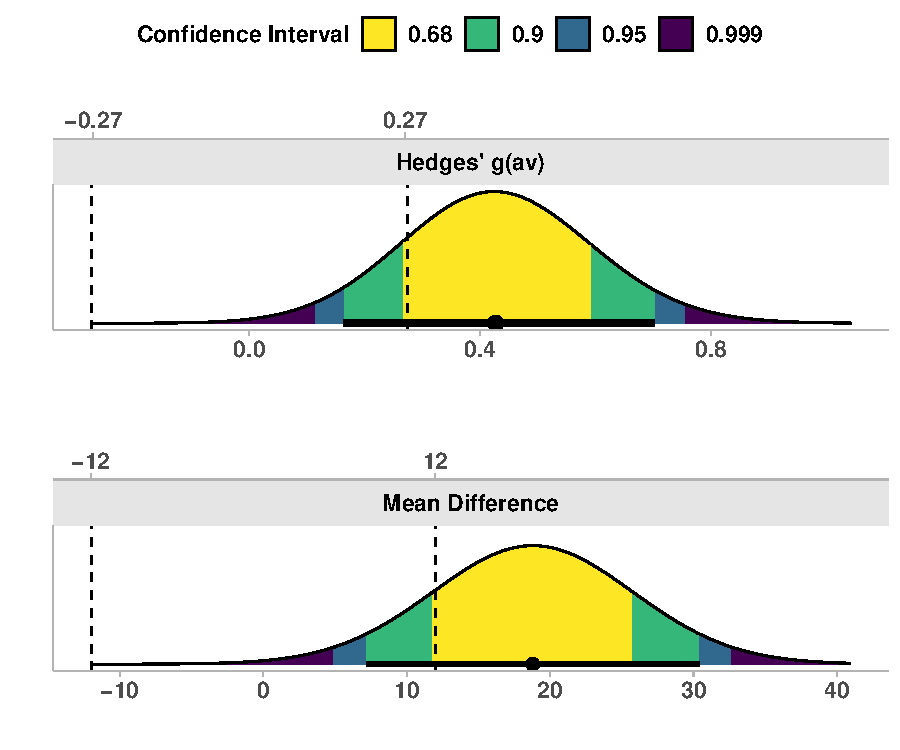
\includegraphics{tenan_arc_manuscript_files/figure-latex/unnamed-chunk-2-1.pdf}
\caption{A visualization of the cumulative distribution function with 4
levels of confidence being displayed for the standardized mean
difference (top panel) and the mean difference (bottom panel)}
\end{figure}

The interpretation provided above takes a Neyman-Pearson perspective.
Both the NHST and TOST tests have an alpha-level of 0.05 and one reached
significance will the other did not. Therefore, an author using this
approach would have to conclude that one null hypothesis is rejected
regarding GLU while other other null hypothesis is rejected.

However, those who wish to use an estimation approach may have a
different interpretation. Under the approach outlined by Rafi \&
Greenland (\protect\hyperlink{ref-rafi2020}{2020}), we could instead
look at the data and see how ``compatible'' the data is with each
competing hypothesis (i.e., NHST versus TOST). From this perspective,
the interpretation is much more fluid, and one could conclude that the
data is more incompatible with ``no effect'' than ``equivalence''
(p-values of 0.008 and 0.83, respectively).

Both perspectives are valid and it is up to researchers to decide how
they plan to tests or estimate their effects. Again, it our belief that
researchers, not editorial boards, are usually the better judges of what
statistical framework is best for their research questions. However,
researchers should be consistent with whatever language/framework (e.g.,
estimation or NHST) within each study/manuscript.

\newpage

\hypertarget{references}{%
\section*{References}\label{references}}
\addcontentsline{toc}{section}{References}

\hypertarget{refs}{}
\begin{CSLReferences}{1}{0}
\leavevmode\vadjust pre{\hypertarget{ref-altman2003}{}}%
Altman, D. G. (2003). Statistics notes: Interaction revisited: The
difference between two estimates. \emph{BMJ}, \emph{326}(7382),
219--219. \url{https://doi.org/10.1136/bmj.326.7382.219}

\leavevmode\vadjust pre{\hypertarget{ref-altman2011}{}}%
Altman, D. G., \& Bland, J. M. (2011). How to obtain the confidence
interval from a p value. \emph{BMJ}, \emph{343}(aug08 1), 2090--2090.
\url{https://doi.org/10.1136/bmj.d2090}

\leavevmode\vadjust pre{\hypertarget{ref-boos}{}}%
Boos, D. D., \& Stefanski, L. A. (2011). P-value precision and
reproducibility. \emph{The American Statistician}, \emph{65}(4),
213--221. \url{https://doi.org/10.1198/tas.2011.10129}

\leavevmode\vadjust pre{\hypertarget{ref-caldwell2019}{}}%
Caldwell, A. R., \& Cheuvront, S. N. (2019). Basic statistical
considerations for physiology: The journal temperature toolbox.
\emph{Temperature}, \emph{6}(3), 181--210.
\url{https://doi.org/10.1080/23328940.2019.1624131}

\leavevmode\vadjust pre{\hypertarget{ref-campbell2018}{}}%
Campbell, H., \& Gustafson, P. (2018). Conditional equivalence testing:
An alternative remedy for publication bias. \emph{PLOS ONE},
\emph{13}(4), 0195145.
\url{https://doi.org/10.1371/journal.pone.0195145}

\leavevmode\vadjust pre{\hypertarget{ref-vigex}{}}%
Deyle, G. D., Allen, C. S., Allison, S. C., Gill, N. W., Hando, B. R.,
Petersen, E. J., Dusenberry, D. I., \& Rhon, D. I. (2020). Physical
therapy versus glucocorticoid injection for osteoarthritis of the knee.
\emph{New England Journal of Medicine}, \emph{382}(15), 1420--1429.
\url{https://doi.org/10.1056/NEJMoa1905877}

\leavevmode\vadjust pre{\hypertarget{ref-elkinsres}{}}%
Elkins, M. R., Pinto, R. Z., Verhagen, A., Grygorowicz, M., Soderlund,
A., Guemann, M., Gomez-Conesa, A., Blanton, S., Brismee, J. M., Agarwal,
S., Jette, A., Harms, M., Verheyden, G., \& Sheikh, U. (2022).
Correspondence: Response to lakens. \emph{Journal of Physiotherapy},
\emph{68}(3), 214. \url{https://doi.org/10.1016/j.jphys.2022.06.003}

\leavevmode\vadjust pre{\hypertarget{ref-elkins2022}{}}%
Elkins, M. R., Pinto, R. Z., Verhagen, A., Grygorowicz, M., Soderlund,
A., Guemann, M., Gomez-Conesa, A., Blanton, S., Brismee, J. M., Ardern,
C., Agarwal, S., Jette, A., Karstens, S., Harms, M., Verheyden, G., \&
Sheikh, U. (2022). Statistical inference through estimation:
Recommendations from the international society of physiotherapy journal
editors. \emph{Journal of Physiotherapy}, \emph{68}(1), 1--4.
\url{https://doi.org/10.1016/j.jphys.2021.12.001}

\leavevmode\vadjust pre{\hypertarget{ref-ferreira2018}{}}%
Ferreira, M. (2018). Research note: The smallest worthwhile effect of a
health intervention. \emph{Journal of Physiotherapy}, \emph{64}(4),
272--274. \url{https://doi.org/10.1016/j.jphys.2018.07.008}

\leavevmode\vadjust pre{\hypertarget{ref-cochrane6}{}}%
Higgins, J. P., Li, T., \& Deeks, J. J. (2019). Choosing effect measures
and computing estimates of effect. \emph{Cochrane Handbook for
Systematic Reviews of Interventions}, 143--176.
\url{https://training.cochrane.org/handbook/current/chapter-06}

\leavevmode\vadjust pre{\hypertarget{ref-hoekstra2014}{}}%
Hoekstra, R., Morey, R. D., Rouder, J. N., \& Wagenmakers, E.-J. (2014).
Robust misinterpretation of confidence intervals. \emph{Psychonomic
Bulletin \& Review}, \emph{21}(5), 1157--1164.
\url{https://doi.org/10.3758/s13423-013-0572-3}

\leavevmode\vadjust pre{\hypertarget{ref-hopewell2009}{}}%
Hopewell, S., Loudon, K., Clarke, M. J., Oxman, A. D., \& Dickersin, K.
(2009). Publication bias in clinical trials due to statistical
significance or direction of trial results. \emph{Cochrane Database of
Systematic Reviews}, \emph{1}.
\url{https://doi.org/10.1002/14651858.MR000006.pub3}

\leavevmode\vadjust pre{\hypertarget{ref-lakensres}{}}%
Lakens, D. (2022). Correspondence: Reward, but do not yet require,
interval hypothesis tests. \emph{Journal of Physiotherapy},
\emph{68}(3), 213--214.
\url{https://doi.org/10.1016/j.jphys.2022.06.004}

\leavevmode\vadjust pre{\hypertarget{ref-lakens2018}{}}%
Lakens, D., Scheel, A. M., \& Isager, P. M. (2018). Equivalence testing
for psychological research: A tutorial. \emph{Advances in Methods and
Practices in Psychological Science}, \emph{1}(2), 259--269.
\url{https://doi.org/10.1177/2515245918770963}

\leavevmode\vadjust pre{\hypertarget{ref-lindley}{}}%
Lindley, D. V. (1957). A statistical paradox. \emph{Biometrika},
\emph{44}(1-2), 187--192.
\url{https://doi.org/10.1093/biomet/44.1-2.187}

\leavevmode\vadjust pre{\hypertarget{ref-lohse2020systematic}{}}%
Lohse, K. R., Sainani, K. L., Taylor, J. A., Butson, M. L., Knight, E.
J., \& Vickers, A. J. (2020). Systematic review of the use of
{``magnitude-based inference''} in sports science and medicine.
\emph{PLOS ONE}, \emph{15}(6), e0235318.
\url{https://doi.org/10.1371/journal.pone.0235318}

\leavevmode\vadjust pre{\hypertarget{ref-maier2022}{}}%
Maier, M., \& Lakens, D. (2022). Justify your alpha: A primer on two
practical approaches. \emph{Advances in Methods and Practices in
Psychological Science}, \emph{5}(2), 251524592210803.
\url{https://doi.org/10.1177/25152459221080396}

\leavevmode\vadjust pre{\hypertarget{ref-mayo2021}{}}%
Mayo, D. G. (2021). The statistics wars and intellectual conflicts of
interest. \emph{Conservation Biology}.
\url{https://doi.org/10.1111/cobi.13861}

\leavevmode\vadjust pre{\hypertarget{ref-mazzolari2022}{}}%
Mazzolari, R., Porcelli, S., Bishop, D. J., \& Lakens, D. (2022).
\emph{Myths and methodologies: The use of equivalence and
non-inferiority tests for interventional studies in exercise physiology
and sport science} {[}Experimental Physiology.{]}.
\url{https://doi.org/10.1113/ep090171}

\leavevmode\vadjust pre{\hypertarget{ref-morey2015}{}}%
Morey, R. D., Hoekstra, R., Rouder, J. N., Lee, M. D., \& Wagenmakers,
E.-J. (2015). The fallacy of placing confidence in confidence intervals.
\emph{Psychonomic Bulletin \& Review}, \emph{23}(1), 103--123.
\url{https://doi.org/10.3758/s13423-015-0947-8}

\leavevmode\vadjust pre{\hypertarget{ref-rafi2020}{}}%
Rafi, Z., \& Greenland, S. (2020). Semantic and cognitive tools to aid
statistical science: Replace confidence and significance by
compatibility and surprise. \emph{BMC Medical Research Methodology},
\emph{20}(1). \url{https://doi.org/10.1186/s12874-020-01105-9}

\leavevmode\vadjust pre{\hypertarget{ref-rouder2009bayesian}{}}%
Rouder, J. N., Speckman, P. L., Sun, D., Morey, R. D., \& Iverson, G.
(2009). Bayesian t tests for accepting and rejecting the null
hypothesis. \emph{Psychonomic Bulletin \& Review}, \emph{16}(2),
225--237.

\leavevmode\vadjust pre{\hypertarget{ref-sainani2020}{}}%
Sainani, K. L., Borg, D. N., Caldwell, A. R., Butson, M. L., Tenan, M.
S., Vickers, A. J., Vigotsky, A. D., Warmenhoven, J., Nguyen, R., Lohse,
K. R., Knight, E. J., \& Bargary, N. (2020). Call to increase
statistical collaboration in sports science, sport and exercise medicine
and sports physiotherapy. \emph{British Journal of Sports Medicine},
\emph{55}(2), 118--122.
\url{https://doi.org/10.1136/bjsports-2020-102607}

\leavevmode\vadjust pre{\hypertarget{ref-senn2005dichotomania}{}}%
Senn, S. (2005). Dichotomania: An obsessive compulsive disorder that is
badly affecting the quality of analysis of pharmaceutical trials.
\emph{Proceedings of the International Statistical Institute, 55th
Session}.
\url{https://www.isi-web.org/isi.cbs.nl/iamamember/CD6-Sydney2005/ISI2005_Papers/398.pdf}

\leavevmode\vadjust pre{\hypertarget{ref-tenan2020}{}}%
Tenan, M. S., Simon, J. E., Robins, R. J., Lee, I., Sheean, A. J., \&
Dickens, J. F. (2020). Anchored minimal clinically important difference
metrics: Considerations for bias and regression to the mean.
\emph{Journal of Athletic Training}, \emph{56}(9), 1042--1049.
\url{https://doi.org/10.4085/1062-6050-0368.20}

\end{CSLReferences}

%
%
%\aucontribute{}

%
%
%
%


\end{document}
